%!TEX root = ../DevaramaniS-[RnD-MT]Report.tex

\chapter{State of the Art}
%\section{....}
%Use as many sections as you need in your related work to group content into logical groups
%
%correctly cite your sources \cite{art1}.

The current state of the art focuses on various approaches to implement complex robot tasks involving robust motions and complex motion primitives. As mentioned earlier (section~\ref{chap:Intro}), the task requirements impose explicit constraints on robot motions. These constraints indicate the desired force or motion to be executed by the robot. It is imperative to consider the dynamic properties of the system to realize these constraints instantaneously and execute the optimal motions. In this section, current state of the art relating to robot dynamic algorithms, task specification formalisms and dynamic solvers are summarized briefly.

\section{Robot dynamics algorithms}
Robot dynamics deals with the relationship between applied force and produced accelerations in the system~\cite{featherstone2014rigid}. The robot dynamics algorithms refer to numerical computations of quantities associated with dynamics. It is well known that the robot dynamics problem is of two types -  forward and inverse dynamics. The forces applied on any rigid body produces acceleration in the direction of applied force, this is termed as \textit{forward dynamics}. The equation used to solve forward dynamics problem is given by~\cite{featherstone2014rigid},
\begin{equation}\label{eq:fd}
	FD \rightarrow M(q)^{-1} (\tau - C(q, \dot{q})) = \ddot{q}
\end{equation}

where, $M(q)$ stands for inertia matrix represented in joint space and is a function of joint position ($q$). $\tau$ denotes the applied force and $C$ is the Centrifugal and Coriolis forces acting on the system. 
 The \textit{inverse dynamics} deals with computation of forces required to produce the desired acceleration. The equation used to solve inverse dynamics problem can be formulated as~\cite{vukcevic2018extending}~\cite{featherstone2014rigid},

\begin{equation}
	\label{eq:ID}
	ID \rightarrow M(q)\ddot{q} + C(q, \ddot{q}) = \tau
\end{equation}

The above equation is also termed as \textit{dynamic equation of motion} for rigid body system (further explanation can be found in appendix~\ref{chap:dynamic}). There are several types of robots such as manipulators, mobile robots, aerial robots etc, which are composition of rigid bodies. In this project, to simplify the analysis of robot dynamics, \textit{Spatial notations} are used to represent the system and follows the convention as used in Featherstone~\cite{featherstone2014rigid}. The Spatial notions include 6D vectors describing six degrees of freedom of a single rigid body. 

The applications of forward dynamics can be found mainly in simulation, whereas, inverse dynamics is applied for motion control system~\cite{featherstone1984robot}. However, there are different robot task definitions that requires combination of forward and inverse dynamics. Specifically for applications involving \textit{posture control} (humanoid robots and manipulators), the robot must realize the motion and force constraints instantaneously as imposed by the task requirements. The basic algorithms to solve each of the dynamics problem are listed below,
\begin{enumerate}
	\item \textit{Forward dynamics}
	\begin{itemize}
		\item \textit{Composite Rigid Body Algorithm (\hyperref[crba]{CRBA})}~\cite{walker1982efficient}: For the given link length, $n < 9$, this method is an efficient algorithm than \hyperref[aba]{ABA}, to compute forward dynamics~\cite{featherstone2000robot}. 
		\item  \textit{Articulated-Body Algorithm (\hyperref[aba]{ABA})}: The method considers whole system as articulated body and computes the forward dynamics and has \textit{O(n)} computational complexity.
	\end{itemize}
	\item \textit{Inverse dynamics}
	\begin{itemize}
		\item \textit{Recursive Newton-Euler Algorithm (\hyperref[rnea]{RNEA})}: The algorithm is applied to calculate inverse dynamics of a general kinematic tree~\cite{featherstone2000robot}. It involves two passes - \textit{outward} and \textit{inward}. In outward pass, \textit{velocity} and \textit{acceleration} quantities are computed from base to the leaves and \textit{joint forces} are computed from leaves to the root during inward pass~\cite{featherstone2014rigid}. 
	\end{itemize}
	\item \textit{Hybrid dynamics}
	\begin{itemize}
		\item \textit{Articulated-Body Hybrid Dynamics Algorithm} - 
		\item \textit{Popov-Vereshchagin Hybrid Dynamic Algorithm} - 
	\end{itemize}
	
	
\end{enumerate}
 
The State of the art section discusses the various software frameworks and dynamic solvers employed in robot manipulators to dynamically realize constraints originating from task specification. 

The kinematic and dynamic solvers compute control inputs for a manipulator given the manipulator’s dynamic parameters such as link inertia or joint friction, and external forces acting on the manipulator. They realize the task constraints that originate from task specification. Similarly, a mobile base naturally resembles a partially-constrained floating base. The constrained degrees of freedom of motions are,
\begin{itemize}
	\item linear acceleration perpendicular to the ground;
	\item angular acceleration about the two axes that are parallel to the ground.
\end{itemize}

Additionally, each wheel introduces a \textit{Cartesian acceleration constraint} known as the \textit{sliding constraint}. In order to realize these motion constraints in mobile robots, the paper presents an extension to \textbf{Popov-Vereshchagin} hybrid dynamic solver. The solver computes the stabilized control inputs in manipulators, given the task objectives, the motion model of the robot as well as the cost function. The previous methods to address the navigation problem such as path tracking, point-point stabilization etc were controlled at kinematic level. There are few current approaches that explicitly control the robot at a dynamic level. One of the papers addresses the general problem of path tracking in mobile robots by presenting a detailed dynamic model with torque coupling. But the article fails to address the complex inner loop dynamics.


\section{Software Frameworks}

\subsection{Task Frame Formalism (TFF)}

TFF is an intuitive programming framework for manipulator applications. It is part of the robot control architecture to transform the high-level commands to unambiguous low-level control parameters current approaches aim at executing complex robot tasks by specifying various compliant motion commands for manipulators. These high-level commands have to be interpreted as atomic robot actions, i.e. no further subdivision is possible. The implementations are primarily focused in the field of the robot manipulator. Manipulation primitives can be linked together to a sequence or complex nets, which describe a robot task. By the execution of these primitives, a huge variety of very complex robot tasks can be covered [3]-[6]. \\ 
Within this framework, the whole space of possible task directions can be divided into two orthogonal subspaces: one composed of force-controlled directions (position-constrained), and the other that represents velocity-controlled directions (force-constrained). A great number of tasks can be performed within this framework. The only condition is that it must be possible to decompose the task into force and velocity- controlled directions. \\ 

The drawback of the task frame approach is that it only applies to task geometries for which separate control modes can be assigned independently to three pure translational and three pure rotational directions along the axes of a single frame. A more systematic approach is to assign control modes and corresponding constraints to arbitrary directions in the six-dimensional manipulation space.

\subsection{Operational Space Formulation}
The operational space of a manipulator is defined by the configuration space of the end-effector (the standard cartesian space). Operational space control (OSC) is an approach to manipulator control that focuses on the dynamic behavior of a serial rigid-link manipulator as seen at the end effector as it evolves in its operational space [7]. \\ The description, analysis, and control of manipulator systems with respect to the dynamic characteristics of their end-effectors have been the basic motivation in the research and development of the operational space formulation framework [8]. \\ An operational coordinate system is a set of x of m independent parameters describing the manipulator end-effector position and orientation in the frame R0. The end-effector equations of motion in operational space are [9],\\
\textbf{$$ \lambda(q) \ddot{x} + \mu (q, \dot q) + p(q) = F_{op} $$}
Where, $\lambda (q)$ is the kinetic energy matrix of the system with respect to the operational point. $x$ defines the operational space coordinates of the end-effector.\\	
$\mu (q, \dot q)$ represents the Coriolis and centrifugal forces acting at the same operational point. $p(q)$ depicts the gravitational forces also expressed at that point.	$F_{op}$ is the generalized force vector expressed in the operational space.


One drawback of the approach is that it directly controls the manipulator in its functional / task space rather than controlling in corresponding joint space that occurs only after geometric and kinematic transformations [10].

\subsection{Stack of Tasks(SoT)}{.....}

\subsection{Instantaneous task specification using constraints (iTaSC)}
(De Schutter et al.) was the first to introduce a systematic constraint-based procedure to specify complex tasks for a variety of sensor-based robotic systems [1].

\begin{figure}[h!]
	\centering
	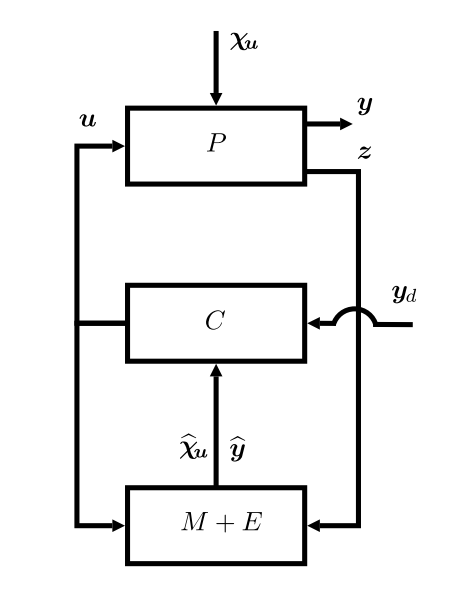
\includegraphics[scale=0.5]{images/General-control-scheme.png}
\end{figure}
The iTaSC is a is a systematic constraint-based approach to specify complex tasks of general sensor-based robot systems. iTASC integrates both instantaneous task specification and estimation of geometric uncertainty in a unified framework. It allows easy specification and code-generation for robot tasks. It generates robot motions by specifying constraints between (parts of) the robots and their environment. iTaSC was born as a specification formalisms to generalize and extend existing approaches, such as the Operational Space Approach, the Task Function Approach, the Task Frame Formalism, geometric Cartesian Space control, and Joint Space control.

The key advantages of iTaSC over traditional motion specification methodologies are [11]:
\begin{itemize}
	\item \textit{Composability of constraints: }Multiple constraints can be combined, hence the constraints can be partial, i.e. they do not have to constrain the full 6D relation between two objects.
	\item \textit{Re-usability of constraint specification:} The constraints specify a relation between feature frames, which have a semantic meaning in the context of a task, implying that the same task specification can be reused on different objects.
	\item \textit{Automatic derivation of the control solution:} The iTaSC methodology generates a robot motion that optimizes the constraints by automatically deriving the controllers from the constraint specification.
\end{itemize}
The iTaSC concepts apply to specifications in the robot, Cartesian and sensor space, to the position, velocity or torque-controlled robots, to explicit and implicit specifications, and to equality and inequality constraints. The current implementation, however, is currently still limited to the velocity control and equality constraints subset.

\section{Software architecture}
\subsection{Whole body control}{....}

\section{Limitations of previous work}

\textbf{Software frameworks: }The primitive software frameworks implemented in the area of robot manipulators to handle the constraints originating from task specification are,
\begin{itemize}
\item Task frame formalism(TFF)
\item The Operational Space Formulation
\item Instantaneous task specification using constraints(iTaSC)
\item Stack Of Tasks(SOT)
\end{itemize}


